\chapter{Einleitung}
In der Astrophysik werden Objekte untersucht, die weder beeinflusst, noch kontrolliert oder isoliert beobachtet werden können.
Astrophysiker sind darauf angewiesen, die begrenzten kosmischen Experimente ihrer Zeit passiv zu beobachten. 
FACT übernimmt dabei unter anderem die Aufgabe, mehrere kosmische Strahlungsquellen zu beobachten und bei Anomalien größere Teleskope für die genauere Observation der Ereignisse zu informieren. 

Im Feld der Astroteilchenphysik werden verschiedene Quellen im Weltraum observiert.
Ziel der Observationen ist es, ein tiefgreifendes Verständnis über deren Entstehung sowie die dominierenden Wechselwikungsprozesse zu erlangen. 
Quellen kosmischer Strahlung sind überwiegend aktive galaktische Kerne, Neutronensterne und Supernova-Überreste. 
Die Energien der Teilchen decken ein Spektrum von \SI{e7}{\electronvolt} bei solarer kosmischer Strahlung bis zu \SI{e20}{\electronvolt} bei extragalaktischer kosmischer Strahlung ab. 

\begin{figure}
  \centering
  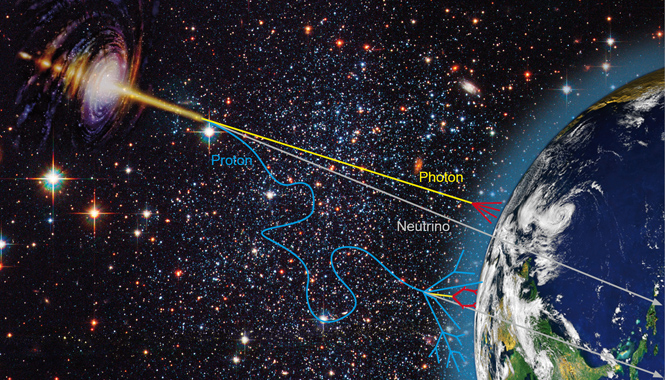
\includegraphics[width=0.7\textwidth]{./images/sources-detection.jpg}
  \caption{Möglicher Weg der drei Teilchenklassen von der Quelle bis zu ihrer Detektion \cite{overview-detec}.}
\end{figure}

Auf die Erdatmosphäre treffen pro Sekunde und Quadratmeter durchschnittlich in etwa \num{e3} Teilchen~\cite{gaisser}.
Diese produzieren je nach Teilchenart und Energie Schauer, in denen viele Sekundärteilchen erzeugt werden. 
Je nach Teilchenart gibt es verschiedene Detektionsmöglichkeiten, wovon FACT eine erdbasierte Variante für $\gamma$-Quanten und Hadronen nutzt. 
Die kosmischen Teilchen lassen sich in drei verschiedene Klassen einteilen. 
Dabei zählt der Sonnenwind zu einer der ständigen Quellen, durch die geladene kosmische Strahlung auf die Erdatmosphäre trifft.

\section*{Geladene kosmische Strahlung}
Geladene kosmische Strahlung besteht überwiegend aus Protonen, Heliumkernen und freien Elektronen. 
Aufgrund ihrer Ladung verliert sie jegliche Richtungsinformation durch Magnetfelder. 
Dies hat zur Folge, dass die Erde isotrop von geladener Strahlung getroffen wird.
Die geladene Strahlung tritt wesentlich häufiger auf, als die Ungeladene. 

\section*{Photonen}
Photonen sind ungeladen, sodass eine Richtungsrekonstruktion mit ihnen möglich ist. 
Jedoch kommt es beim Eindringen der Teilchen in die Erdatmosphäre zur Schauerbildung, sodass die Richtungsrekonstruktion nicht trivial ist. 
Das aufschauern vor dem Detektor kann vermieden werden, indem Satelliten in die Erdumlaufbahn gebracht werden wie es zum Beispiel beim Fermi Gamma-ray Space Telescope~\cite{fermi} der Fall ist.

\section*{Neutrinos}
Aufgrund ihrer elektrischen Neutralität sowie ihres geringen Wirkungsquerschnitts liefern auch Neutrinos Informationen über die Quellregionen. 
Zum Nachweis von astrophysikalischen Neutrinos werden, aufgrund ihrer geringen Wechselwirkungswahrscheinlichkeit, große Detektorvolumina wie zum Beispiel das IceCube Experiment benötigt.
Da ein direkter Nachweis bis jetzt nicht möglich ist, wird beim IceCube Experiment \cite{icecube} der Cherenkov-Effekt im Eis genutzt, um über indirekte Strahlung Neutrinos nachzuweisen.
